\section{November 28, 2022}

\subsection{Geometries and linear groups}

We have a number of different infinite matrix groups:
\[GL_n, SL_n, O_n, U_n,\hdots\] 
over infinite fields:
\[\RR\text{ (reals)}, \CC\text{ (complex)}, \HH\text{ (quaternions)}, \hdots \]

For the next few lectures, we'll spend some time focusing on better understanding these matrix groups over these fields. Which groups are out there? What is their structure?

In $1872$, Felix Klein proposed the \ac{Erlangen Program}: that studying geometries is somehow equivalent to studying different groups of symmetries. 

One example that we have already studied in depth is the group of isometries: 
\[\text{Euclidean geometries in }\RR^n \longleftrightarrow M_n = O_n(\RR)\ltimes \RR^n.\]

Here are some others:

\begin{example}
\exlabel 

$O_{p,q}(\RR)$ is the symmetry group of the form with signature $(p,0,q)$. In other words, 

\[O_{p,q}(\RR) = \Bigg\{A \in \GL_n(\RR) : \underbrace{A^t\twotwo{I_p}{0}{0}{-I_q}A = \twotwo{I_p}{0}{0}{-I_q}}_{A\text{ preserves the form w/ this matrix}}\Bigg\}.\]
\end{example}

$O_{n,0}(\RR)$ is the usual orthogonal group. $O_{3,1}(\RR)$ plays an important role in Lorentz transformations and hyperbolic geometries (equations of the form $x^2+y^2+z^2-t^2$). 

\begin{example}
\exlabel
\[SO_2(\RR)\cong \RR/(2\pi \ZZ) \cong \{z\in \CC : \vert z\vert =1\}.\]
\end{example}

In other words, we can think about $SO_2(\RR)$ as the unit circle in the complex plane. Its noteworthy that this group is abelian, which is sort of lucky and does not generalize. This group is important to understand, but a bit simple, so let's see what happens in higher dimensions.

\begin{example}
\exlabel

What does $SO_3$ look like geometrically?
\end{example}

How to describe elements of $SO_3(\RR)$: 
\begin{itemize}
    \item Pick a rotation axis $a\in \RR^3$, $\vert a\vert = 1$
    \item Pick an angle $\theta$ to rotate about our pole
\end{itemize}

This leads us to a few intuitive characterizations for the geometry of $SO_3$.
\begin{definition}
\deflabel

An \ac{$n$-sphere} is a set of points 
\[S^n = \{a\in \RR^{n+1} : \vert a\vert = 1\}.\]
\end{definition} 

We define it this way because an $n$-sphere is a topologically $n$-dimensional object embedded in an $(n+1)$-dimensional space. For example, the surface of a $2$-sphere is $2$-dimensional, but the sphere itself is embedded in $3$-dimensional space.

The characterization for $SO_3$ above amounts to choosing two elements, one from $S^2$, and one from $S^1$. Does this mean that $SO_3(\RR)$ is topologically equivalent to $S^2\times S^1$? The answer is no:

\begin{itemize}
    \item If $\theta = 0$, all $a$ are equivalent (non-unique identity)
    \item $(a, \theta)$ is equal to $(-a, -\theta)$. 
\end{itemize}

What if we try to instead define $a$ from two angles (e.g., think polar coordinates)? This gives a description of any element in $SO_3$ as a combination of three angles, which are also called \ac{Euler angles}. It turns out that $SO_3$ can't be characterized by $(S^1)^3$ either, for reasons that are similar to the first. We can try to visualize degenerate cases with an analogy to a concept in engineering: 

\begin{center}
\begin{asy}
import graph; size(3cm); 
pen dps = linewidth(0.7) + fontsize(10); defaultpen(dps);
pen bronze = RGB(205, 127, 50);
real eps = 10;
real yscaling = 0.75;

path A = scale(3)*unitcircle;
path B = scale(2)*unitcircle;
path C = unitcircle;
path D = scale(0.5)*unitcircle;
draw(A);
draw(B);
draw(C);
filldraw(D, green, green);

draw((0,3)--(0,4), bronze);
draw((0,-3)--(0,-4), bronze);
draw((2,0)--(3,0), bronze);
draw((-2,0)--(-3,0), bronze);
draw((0,1)--(0,2), bronze);
draw((0,-1)--(0,-2), bronze);

path rotation = arc((0,3.4/yscaling), 1, -225+eps, 45-eps);
draw(yscale(yscaling)*rotation, Arrow(3bp));
\end{asy}
\end{center}

Each ring here is called a \ac{gimbal}, which is mounted to an axis by which it can rotate. The direction of rotation for the outermost gimbal is shown, with each subsequent gimbal having alternating perpendicular axes of rotation.

Now, we mount an object inside of our gimbals. Prof. Cohn used a frog, so we'll use a green circle here. This set of three gimbals should in principal allow the frog to achieve any orientation, with each orientation of the frog corresponding to a unique set of three angles of the gimbals. This would be analogous to $SO_3$ being topologically equivalent to $(S^1)^3$. In practice, there are some degenerate cases, like in the illustration, when all three gimbals are aligned so that the configuration is two-dimensional. In this configuration, there is no immediate way to rotate the frog with respect to a pole going directly into/out of the page, which is a problem known as \ac{gimbal lock}. Ultimately, this shows that $SO_3$ can't be equivalent to $(S^1)^3$. 

\subsection{Fundamental Groups}

\begin{definition}
\deflabel

Given a topological space $X$, and some point $x_0\in X$, the \ac{fundamental group} for this point in space is defined as the set 
\[\pi_1(X, x_0) = \{\text{loops based at }x_0\text{ up to deformation}\},\]
with the composition group action.
\end{definition}

A ``loop'' is a closed path. The fundamental group counts paths which are deformed in some way as the same path. 

\begin{figure}[H]
    \centering
    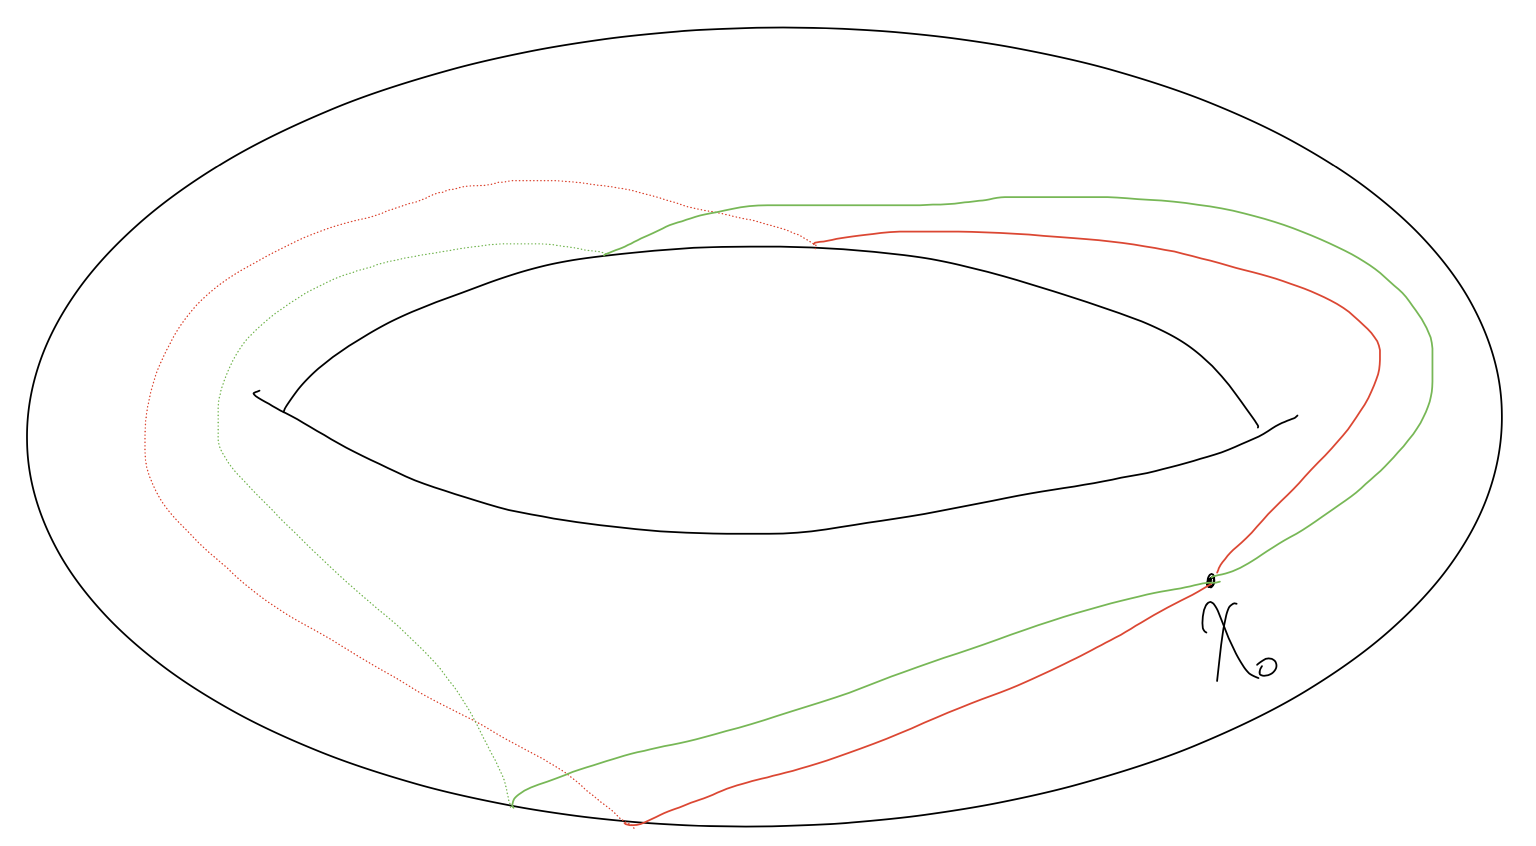
\includegraphics[width=5cm]{images/torus.png}
\end{figure}

For example, the red and green loops on this torus are considered the same, because they have the same fundamental structure, they're just ``deformed''.

\begin{example}
\exlabel
\[\pi_1(S^1, \star) \cong \ZZ.\]
\end{example}

(We use $\star$ for our element because it does not matter where we start our loop). The identity of this group is ``do nothing''. Each element in the group is some integer number of rotations starting and ending at this point, so we have a single generator, going around the circle once. 

\begin{example}
\exlabel
\[\pi_1(\text{torus}, \star) \cong \ZZ^2.\]
\end{example}

The two generators are the number of times the loop goes around the donut, and the number of times the loop goes around the ring of the donut. 

\begin{example}
\exlabel 
\[\pi_1(SO_3(\RR), I)\cong \ZZ/2\ZZ.\]
\end{example}

Prof. Cohn demonstrates this by holding his phone flat in one hand, and rotating it by a full loop, which results in his arm being twisted $180^{\circ}$. Composing this rotation with itself does not result in his arm being ``twice as twisted'', but instead it results in his arm returning to its normal position. In this way, there is no way for his arm to become ``twice as twisted'' once it returns to its identity position; rather, it just untwists itself, which gives some intuition for why the fundamental group is $\ZZ/ 2\ZZ$. 

\subsection{Cubes in $\RR^n$}
\hspace{4.75cm}
\begin{asy}
import graph; size(2cm); 
pen dps = linewidth(0.7) + fontsize(10); defaultpen(dps);
pen dotstyle = black;

pair A = (0,0);
pair B = (0,1);

draw(A--B); 
dot(A);
dot(B);
\end{asy}
\hspace{3.5cm}
\begin{asy}
import graph; size(2cm); 
pen dps = linewidth(0.7) + fontsize(10); defaultpen(dps);
pen dotstyle = black;

pair A = (0,0);
pair B = (0,1);
pair C = (1,1);
pair D = (1,0);

draw(A--B--C--D--cycle);
dot(A);
dot(B);
dot(C);
dot(D);
\end{asy}

\hfill{$n=1$}\hfill{$n=2$}\hfill\hfill

\V

\hspace{3.25cm}
\begin{asy}
import graph; size(2cm); 
pen dps = linewidth(0.7) + fontsize(10); defaultpen(dps);
pen dotstyle = black;

pair A = (-0.5,0.5);
pair B = (0.5,0.5);
pair C = (0.5,-0.5);
pair D = (-0.5,-0.5);
pair E = A/2;
pair F = B/2;
pair G = C/2;
pair H = D/2;

draw(A--B--C--D--cycle);
draw(E--F--G--H--cycle);
draw(A--E);
draw(B--F);
draw(C--G);
draw(D--H);
dot(A);
dot(B);
dot(C);
dot(D);
dot(E);
dot(F);
dot(G);
dot(H);
\end{asy}
\hspace{2.2cm}
\begin{asy}
import graph; size(2.5cm); 
pen dps = linewidth(0.7) + fontsize(10); defaultpen(dps);
pen dotstyle = 3+black;
real s = 1.2;
real r = 0.8;

pair A = (-0.5,0.5);
pair B = (0.5,0.5);
pair C = (0.5,-0.5);
pair D = (-0.5,-0.5);
pair E = A/2;
pair F = B/2;
pair G = C/2;
pair H = D/2;

pair A2 = shift(s,r)*A;
pair B2 = shift(s,r)*B;
pair C2 = shift(s,r)*C;
pair D2 = shift(s,r)*D;
pair E2 = shift(s,r)*E;
pair F2 = shift(s,r)*F;
pair G2 = shift(s,r)*G;
pair H2 = shift(s,r)*H;

draw(A--B--C--D--cycle);
draw(E--F--G--H--cycle);
draw(A2--B2--C2--D2--cycle);
draw(E2--F2--G2--H2--cycle);
draw(A--E);
draw(B--F);
draw(C--G);
draw(D--H);
draw(A2--E2);
draw(B2--F2);
draw(C2--G2);
draw(D2--H2);
draw(A--A2);
draw(B--B2);
draw(C--C2);
draw(D--D2);
draw(E--E2);
draw(F--F2);
draw(G--G2);
draw(H--H2);
dot(A, dotstyle);
dot(B, dotstyle);
dot(C, dotstyle);
dot(D, dotstyle);
dot(E, dotstyle);
dot(F, dotstyle);
dot(G, dotstyle);
dot(H, dotstyle);
dot(A2, dotstyle);
dot(B2, dotstyle);
dot(C2, dotstyle);
dot(D2, dotstyle);
dot(E2, dotstyle);
dot(F2, dotstyle);
dot(G2, dotstyle);
dot(H2, dotstyle);
\end{asy}

\hfill{$n=3$}\hfill{$n=4$}\hfill\hfill

Moving up from one dimension to the next can be thought of as shifting over a copy of the current cube, and then connecting corresponding vertices between the original and the copy. Each time we do this, the number of vertices doubles. The number of facets (i.e., the number of $(n-1)$-dimensional faces) increases by $2$, because we get one facet for each of the current facets when the copy is shifted, as well as a new ``front'' and ``back'' end of the new cube. 

In other words, an $n$-dimensional cube has $2^n$ vertices and $2n$ facets. If its side length is $1$, then its diameter is $\sqrt{1^2+1^2+\hdots +1^2} = \sqrt{n}$. Note the exponential growth in the number of vertices, compared to the sublinear growth of the diameter of the cube. A cube in $n=10^6$ dimensions has a really, really large number of vertices, but a diameter of only $1000$, which becomes tricky to visualize, especially given the fact that hypercubes must be convex. 



